\documentclass[14pt]{extbook}
\usepackage{multicol, enumerate, enumitem, hyperref, color, soul, setspace, parskip, fancyhdr} %General Packages
\usepackage{amssymb, amsthm, amsmath, latexsym, units, mathtools} %Math Packages
\everymath{\displaystyle} %All math in Display Style
% Packages with additional options
\usepackage[headsep=0.5cm,headheight=12pt, left=1 in,right= 1 in,top= 1 in,bottom= 1 in]{geometry}
\usepackage[usenames,dvipsnames]{xcolor}
\usepackage{dashrule}  % Package to use the command below to create lines between items
\newcommand{\litem}[1]{\item#1\hspace*{-1cm}\rule{\textwidth}{0.4pt}}
\pagestyle{fancy}
\lhead{Makeup Progress Quiz 3}
\chead{}
\rhead{Version B}
\lfoot{1648-1753}
\cfoot{}
\rfoot{Summer C 2021}
\begin{document}

\begin{enumerate}
\litem{
Determine the domain of the function below.\[ f(x) = \frac{6}{24x^{2} +6 x -9} \]\begin{enumerate}[label=\Alph*.]
\item \( \text{All Real numbers except } x = a \text{ and } x = b, \text{ where } a \in [-2, 0.2] \text{ and } b \in [-0.3, 2.5] \)
\item \( \text{All Real numbers except } x = a \text{ and } x = b, \text{ where } a \in [-12.4, -11.6] \text{ and } b \in [17.4, 19.7] \)
\item \( \text{All Real numbers.} \)
\item \( \text{All Real numbers except } x = a, \text{ where } a \in [-2, 0.2] \)
\item \( \text{All Real numbers except } x = a, \text{ where } a \in [-12.4, -11.6] \)

\end{enumerate} }
\litem{
Solve the rational equation below. Then, choose the interval(s) that the solution(s) belongs to.\[ \frac{5}{-3x -7} + 5 = \frac{6}{9x + 21} \]\begin{enumerate}[label=\Alph*.]
\item \( x \in [2.63,2.81] \)
\item \( x_1 \in [-2.06, -1.55] \text{ and } x_2 \in [1.8,3.8] \)
\item \( x \in [-1.87,-0.87] \)
\item \( x_1 \in [-2.46, -1.99] \text{ and } x_2 \in [-1.87,0.13] \)
\item \( \text{All solutions lead to invalid or complex values in the equation.} \)

\end{enumerate} }
\litem{
Choose the equation of the function graphed below.
\begin{center}
    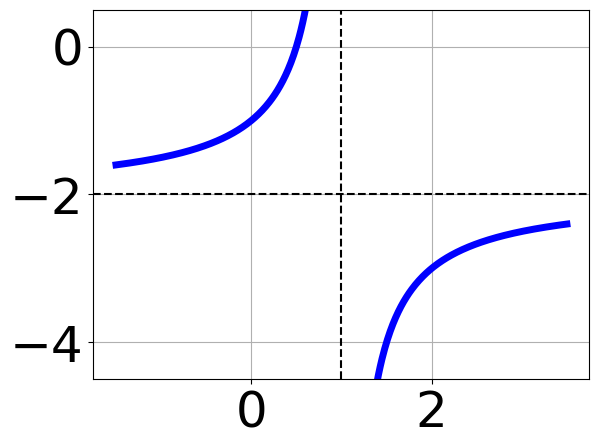
\includegraphics[width=0.5\textwidth]{../Figures/rationalGraphToEquationCopyB.png}
\end{center}
\begin{enumerate}[label=\Alph*.]
\item \( f(x) = \frac{1}{(x - 1)^2} + 4 \)
\item \( f(x) = \frac{1}{x - 1} + 4 \)
\item \( f(x) = \frac{-1}{(x + 1)^2} + 4 \)
\item \( f(x) = \frac{-1}{x + 1} + 4 \)
\item \( \text{None of the above} \)

\end{enumerate} }
\litem{
Choose the graph of the equation below.\[ f(x) = \frac{1}{x + 3} - 1 \]\begin{enumerate}[label=\Alph*.]
\begin{multicols}{2}\item 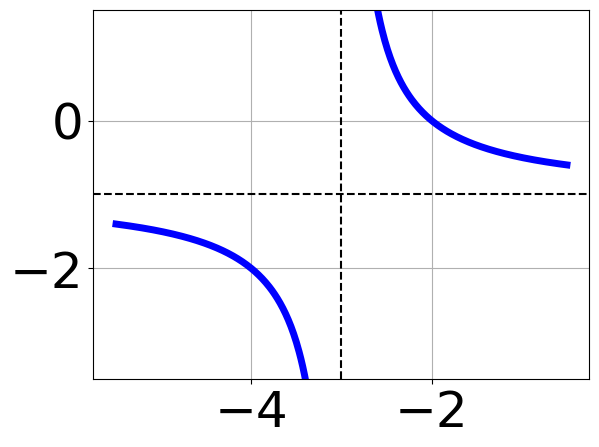
\includegraphics[width = 0.3\textwidth]{../Figures/rationalEquationToGraphCopyAB.png}\item 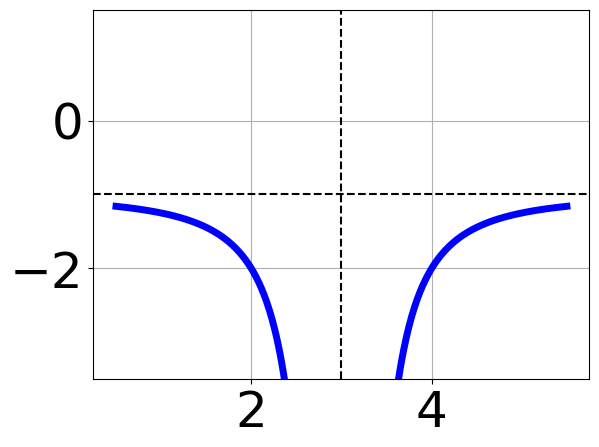
\includegraphics[width = 0.3\textwidth]{../Figures/rationalEquationToGraphCopyBB.png}\item 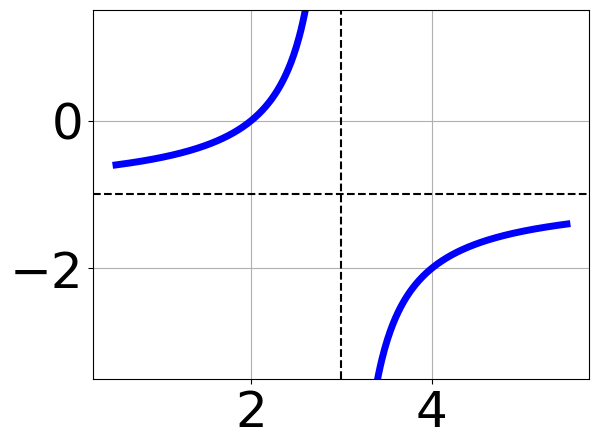
\includegraphics[width = 0.3\textwidth]{../Figures/rationalEquationToGraphCopyCB.png}\item 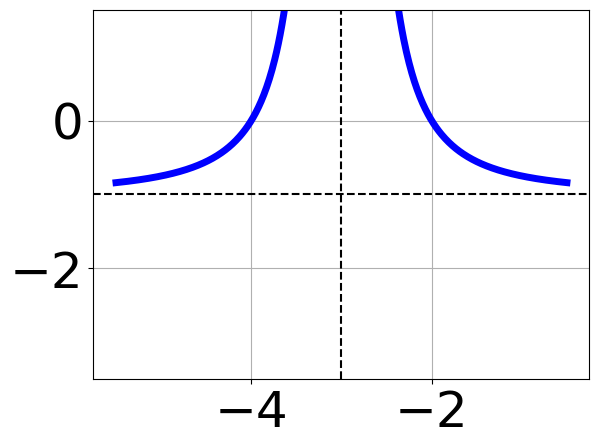
\includegraphics[width = 0.3\textwidth]{../Figures/rationalEquationToGraphCopyDB.png}\end{multicols}\item None of the above.
\end{enumerate} }
\litem{
Determine the domain of the function below.\[ f(x) = \frac{3}{12x^{2} -36 x + 24} \]\begin{enumerate}[label=\Alph*.]
\item \( \text{All Real numbers except } x = a \text{ and } x = b, \text{ where } a \in [14.7, 16.9] \text{ and } b \in [17, 18.2] \)
\item \( \text{All Real numbers except } x = a, \text{ where } a \in [-1.1, 1.7] \)
\item \( \text{All Real numbers except } x = a, \text{ where } a \in [14.7, 16.9] \)
\item \( \text{All Real numbers except } x = a \text{ and } x = b, \text{ where } a \in [-1.1, 1.7] \text{ and } b \in [1.7, 2.9] \)
\item \( \text{All Real numbers.} \)

\end{enumerate} }
\litem{
Solve the rational equation below. Then, choose the interval(s) that the solution(s) belongs to.\[ \frac{3}{5x + 4} + -7 = \frac{2}{-20x -16} \]\begin{enumerate}[label=\Alph*.]
\item \( x \in [0.87,0.94] \)
\item \( x \in [-1.7,1.3] \)
\item \( \text{All solutions lead to invalid or complex values in the equation.} \)
\item \( x_1 \in [-0.7, -0.69] \text{ and } x_2 \in [0.9,5.9] \)
\item \( x_1 \in [-0.79, -0.72] \text{ and } x_2 \in [-0.7,0.3] \)

\end{enumerate} }
\litem{
Choose the graph of the equation below.\[ f(x) = \frac{-1}{x - 2} - 2 \]\begin{enumerate}[label=\Alph*.]
\begin{multicols}{2}\item 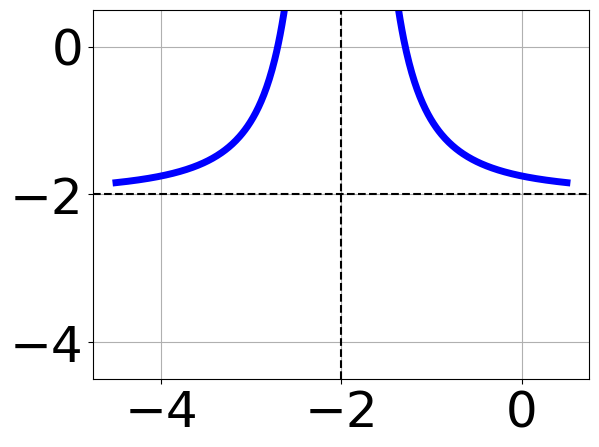
\includegraphics[width = 0.3\textwidth]{../Figures/rationalEquationToGraphAB.png}\item 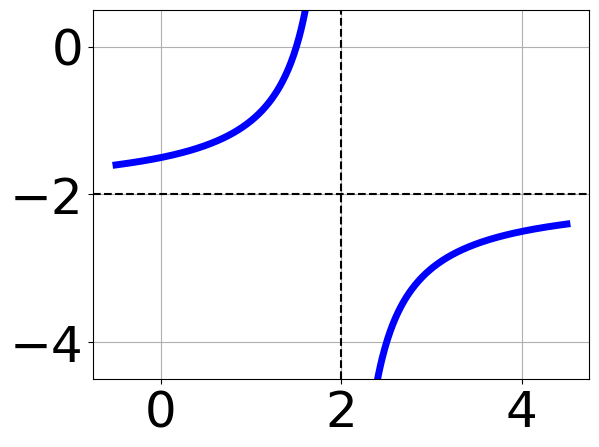
\includegraphics[width = 0.3\textwidth]{../Figures/rationalEquationToGraphBB.png}\item 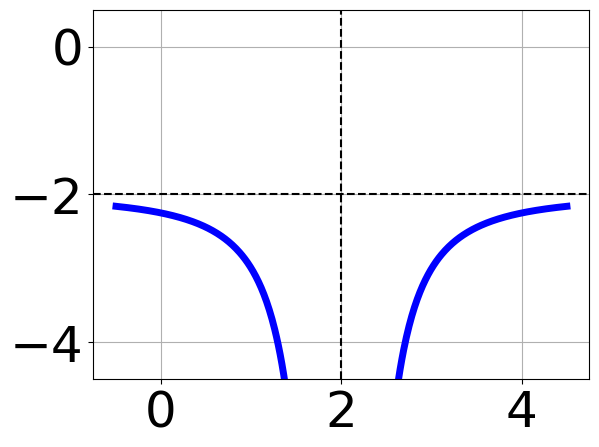
\includegraphics[width = 0.3\textwidth]{../Figures/rationalEquationToGraphCB.png}\item 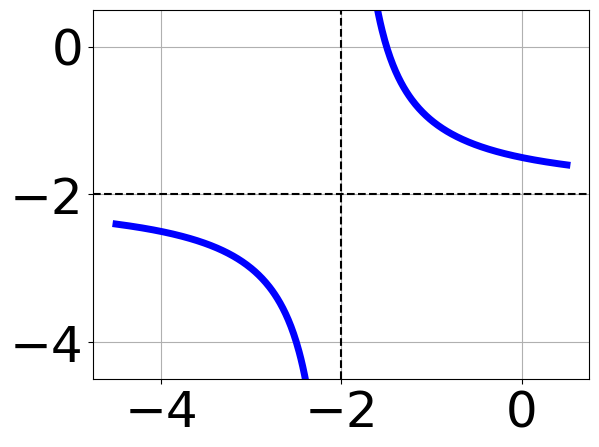
\includegraphics[width = 0.3\textwidth]{../Figures/rationalEquationToGraphDB.png}\end{multicols}\item None of the above.
\end{enumerate} }
\litem{
Choose the equation of the function graphed below.
\begin{center}
    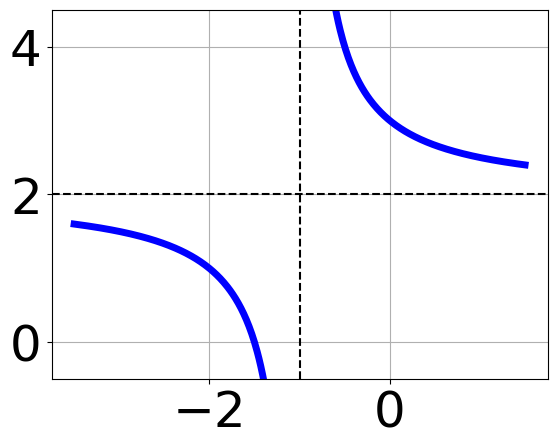
\includegraphics[width=0.5\textwidth]{../Figures/rationalGraphToEquationB.png}
\end{center}
\begin{enumerate}[label=\Alph*.]
\item \( f(x) = \frac{-1}{(x - 1)^2} + 2 \)
\item \( f(x) = \frac{-1}{x - 1} + 2 \)
\item \( f(x) = \frac{1}{x + 1} + 2 \)
\item \( f(x) = \frac{1}{(x + 1)^2} + 2 \)
\item \( \text{None of the above} \)

\end{enumerate} }
\litem{
Solve the rational equation below. Then, choose the interval(s) that the solution(s) belongs to.\[ \frac{5x}{3x + 5} + \frac{-2x^{2}}{18x^{2} +39 x + 15} = \frac{-6}{6x + 3} \]\begin{enumerate}[label=\Alph*.]
\item \( x_1 \in [-2.39, -1.64] \text{ and } x_2 \in [-0.56,-0.38] \)
\item \( x \in [-2.39,-1.64] \)
\item \( x_1 \in [-1.48, -0.61] \text{ and } x_2 \in [-0.17,1.79] \)
\item \( \text{All solutions lead to invalid or complex values in the equation.} \)
\item \( x \in [-0.75,-0.03] \)

\end{enumerate} }
\litem{
Solve the rational equation below. Then, choose the interval(s) that the solution(s) belongs to.\[ \frac{-5x}{2x -6} + \frac{-6x^{2}}{14x^{2} -28 x -42} = \frac{2}{7x + 7} \]\begin{enumerate}[label=\Alph*.]
\item \( \text{All solutions lead to invalid or complex values in the equation.} \)
\item \( x_1 \in [0.16, 0.32] \text{ and } x_2 \in [2,6] \)
\item \( x \in [-1.05,-0.78] \)
\item \( x_1 \in [0.16, 0.32] \text{ and } x_2 \in [-6.2,2.8] \)
\item \( x \in [-1.23,-1.17] \)

\end{enumerate} }
\end{enumerate}

\end{document}